%!TEX root = ../../fourthYearReport.tex


\paragraph{Work package 7 progress}

\begin{figure}
  \centering
    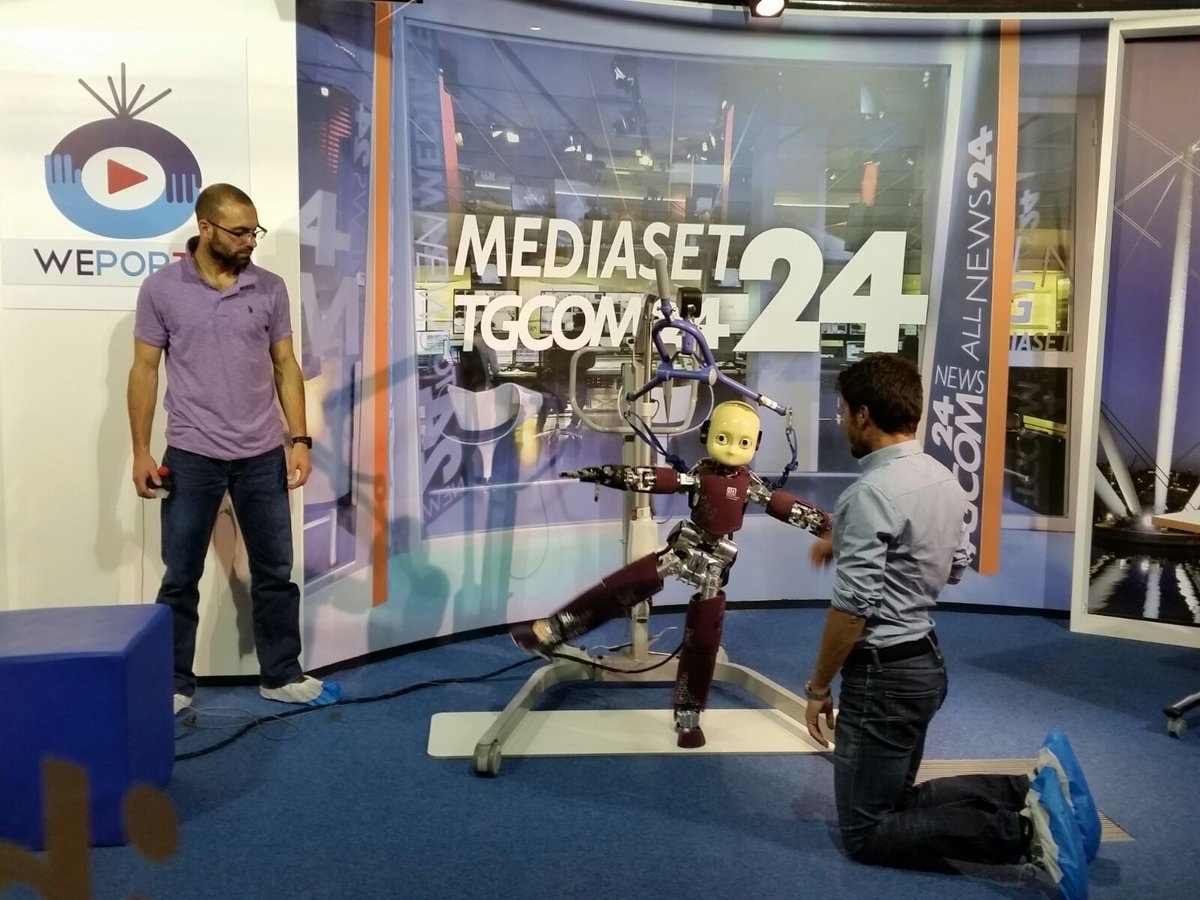
\includegraphics[width=.45\columnwidth]{images/tg24}
    \hspace{1cm}
    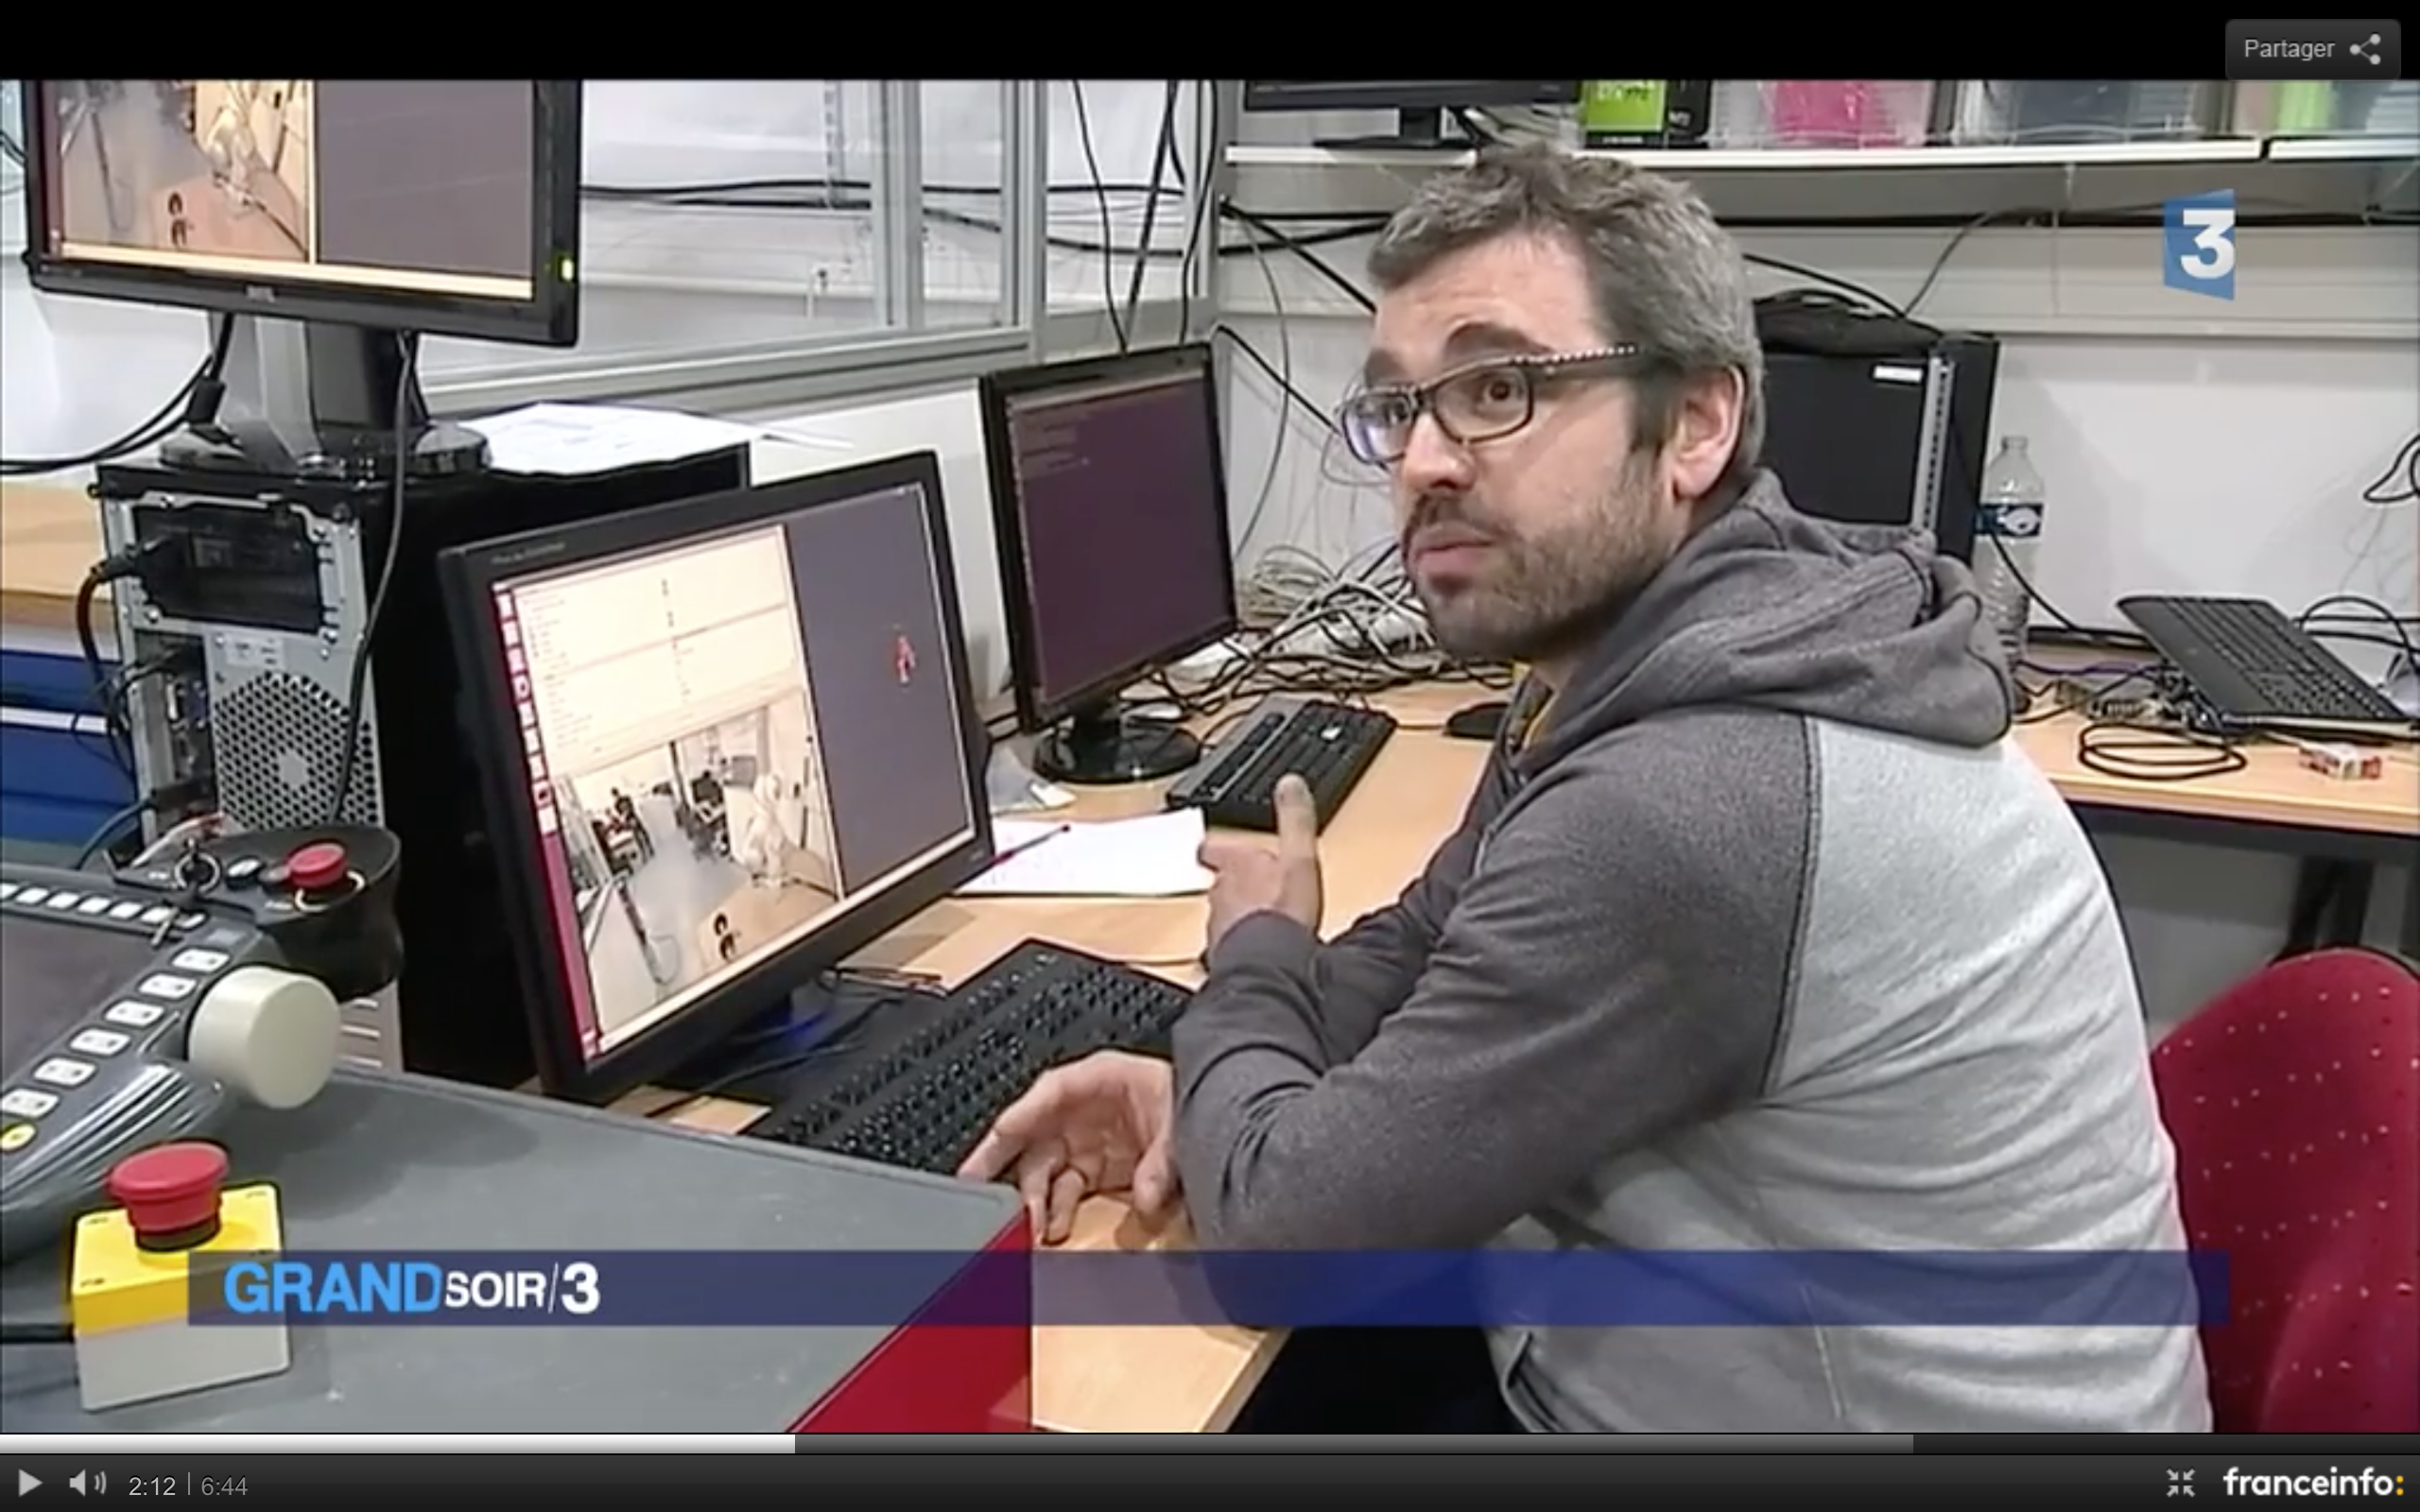
\includegraphics[width=.45\columnwidth]{images/vincent_dissemination}
  \caption{Dissemination of the CoDyCo project was conducted through several events. The left image refers to the
  live event on October 17th, 2016. TgCom24, live tv show on the Italian national channel. The right image
  to a national French television channel (France 3). }
 \label{fig:schemeAlgorithm4}
\end{figure}


Dissemination and exploitation activities included the participation to international events addressed to both commercial and academic institutions. 

\subparagraph{Dissemination activities towards academia, industry, and other users (T7.1)}

Several dissemination activities were conducted during the last year of the project. Here is a
detailed list subdivided by partner.

\begin{itemize}
 \item IIT conducted the following dissemination activities:
 
 \begin{enumerate}
 \item Francesco Nori was invited at the workshop on ``Biomechanics of Anthropomorphic Systems''.
 Toulouse, LAAS-CNRS, November 24-25, 2016. The title of his talk was: ``The geometric foundation
 of the dynamics of physical interaction and AnDy’s roadmap towards proficient human-robot collaboration''.
 \url{https://biomeca-robot.sciencesconf.org/resource/page/id/9}. 
 
 \item Francesco Nori was invited speaker at the Festival della Scienza, Open Science Caf\'e. The title of the 
 presentation was: ``iCub Whole-body Control through Force Regulation on Rigid Noncoplanar Contacts''.
 Genova, November 3rd, 2017.
 
 \item Daniele Pucci was an invited speaker and a selected presentation at the
 ``Workshop on Dynamic Locomotion and Manipulation''. Title of the talk:
 ``A Stable Momentum-Based Controller for Balancing Tasks with Contact Switching''.
 Date: July 13th - 15th. Location: ETH Zurich.
 \url{http://www.dlmc2016.ethz.ch/call-for-abstracts/pleanary-papers.html}.
 
 \item Daniele Pucci was invited speaker in Pontedera. “Locomotion Control for Bipedal Robots”,
 December 19th, 2016: invited at the Center for Micro-BioRobotics, Istituto Italiano di Tecnologia,
 Pontedera, Italy.
 
 \item Francesco Nori was invited professor at INRIA in February. During this period he gave a
 talk on the CoDyCo project on Febraury 5th, 2016.
 
 
 \end{enumerate}
 
 \item TUD conducted the following dissemination activities:
 
 \begin{enumerate}
 \item 2016/05 - Universit\"at Stuttgart, Stuttgart, Germany, host: Marc Toussaint, Machine Learning \& Robotics Lab.
 \item 2016/08 - Max Planck Institute for Intelligent Systems, Tuebingen, Germany, host: Autonomous Motion Department.

 %Elmar
 \item 2016/04 - Technische Universit\"at Graz, Austria. Institute of Neural Engineering, invited by Gernot Mueller-Putz. Title: Probabilistic Models of Human Motor Control for Robotics and Prosthetics. 
 \item 2016/05 - Joanneum Research, Austria. Title: Models of Human Motor Control for Robotics. Guest of Michael Hofbaur, Klagenfurt, Austria.
 \item 2016/11 - University of Zurich, Switzerland. Institute of Neuroinformatics, INI. Title: Probabilistic computational models of human motor control for robot learning. Guest of Shih-Chii Liu. 
 \item 2016/11 - Albert-Ludwigs-Universit\"at Freiburg, Germany. Title: Neural models for brain-machine interfaces and anthropomorphic robotics.
 \item 2017/01 - Frankfurt Institute for Advanced Studies, Germany. Title: Learning to Plan through Reinforcement Learning in Spiking Neural Networks. Guest of Jochen Triesch.  
 \item 2017/02 - Universit\"at L\"ubeck, Germany. Title: Neural models for robot motor skill learning. 

 %Jan
 \item 2016/06 - Sensing: From Minds to Machines, Besheba, Israel.
 \item 2016/09 - 11th Joint Conference on Motor Control \& Learning, Biomechanics \& Training, Darmstadt, Germany.
 \item 2016/09 - 2016 ERNSI Workshop, Treviso, Italy.
 \item 2016/09 - 12th IFIP International Conference on Artificial Intelligence Applications and Innovations (AIAI 2016), Thessaloniki, Greece.
 \item 2016/10 - Okinawa Institute of Technology, Host: K. Doya, Okinawa, Japan.
 \item 2016/11 - HUMANOIDS Workshop: Tactile sensing for manipulation: new progress and challenges, Cancun, Mexico.
 \item 2016/12 - The German-French Conference on Humanoid and Legged Robots (HLR 2016), Tolouse, France.
 \item 2016/12 - Technische Universit\"at Wien, Host: M. Vinzce, Vienna, Germany.

 \end{enumerate}
 
 \item JSI organized a ``Workshop on Human-Robot Collaboration: Towards Co-Adaptive Learning 
 Through Semi-Autonomy and Shared Control'' at IROS 2016, 10 October, Daejeon, Korea. Organizers:
 Luka Peternel (HRI2, ADVR, IIT, Italy) and Guilherme Maeda (IAS, TU Darmstadt, Germany), 
 Leonel Rozo (IIT, Italy), Serena Ivaldi (INRIA Nancy Grand-Est, France), Claudia Pérez D'Arpino (MIT, USA),
 Julie A. Shah (MIT, USA), Jan Babič (JSI, Slovenia), Tamim Asfour (KIT, Germany) 
 and Erhan Oztop (Ozyegin University, Turkey).
 
 \item UPMC conducted the following dissemination activities:
 
 \begin{enumerate}
 \item Nicolas Perrin, ``Abstractions in humanoid motion''. March 6th, 2017: invited seminar at the Algorithmic, Complexity and Logic Laboratory (LACL) of Paris-Est Créteil Val-de-Marne University (UPEC).

 \item Olivier Sigaud, ``From Machine Learning to Deep Learning with a focus on regression and RL''.
 January 24th, 2017: invited seminar at the ONERA internal workshop on machine learning and deep learning

 \item Vincent Padois: ``Vous avez dit robot? Au del\`a du mythe, la r\'ealit\'e...''
 March 22nd, 2016: invited seminar at the CE Industriel d’Air France.
 
 \item Vincent Padois (plenary talk), ``Collaborative robotics : from workspace sharing to physical interactions''
 August 31st, 2016. Plenary talk at the 21th International Conference on Methods and Models in Automation and Robotics.
 
 \end{enumerate}
  
 \item Also, during the fourth year the CoDyCo consortium conducted the following 
 wide audience dissemination activities:
 
 \begin{enumerate}
 \item ``Technologies: les robots envahissent notre quotidien''
 May 26th, 2016: Reportage the for the daily evening news show ``Le Grand Soir 3'' on the national channel France 3. URL : \url{http://www.francetvinfo.fr/internet/technologies-les-robots-envahissent-notre-quotidien_1470757.html}.
 
 \item ``iCub on TgCom24''. October 17th, 2016. Live event with the iCub showing his balancing capabilities during
 a event connected to the Festival della Scienza.
 
 \item The iCub advanced balancing capabilities were on IEEE Spectrum Video Friday twice during 2016. 
 See the yoga++ video  
\url{https://goo.gl/2V3Uzn} and the footstep recovery  \url{https://goo.gl/b2sZmE}.

\item The iCub and CoDyco were on an Italian newspaper. \url{https://goo.gl/xJCrMG}.

 \end{enumerate}
 
\end{itemize}
